
\documentclass[12pt,conference]{IEEEtran}

\ifCLASSINFOpdf
  % \usepackage[pdftex]{graphicx}
  % declare the path(s) where your graphic files are
  % \graphicspath{{../pdf/}{../jpeg/}}
  % and their extensions so you won't have to specify these with
  % every instance of \includegraphics
  % \DeclareGraphicsExtensions{.pdf,.jpeg,.png}
\else
  % or other class option (dvipsone, dvipdf, if not using dvips). graphicx
  % will default to the driver specified in the system graphics.cfg if no
  % driver is specified.
  % \usepackage[dvips]{graphicx}
  % declare the path(s) where your graphic files are
  % \graphicspath{{../eps/}}
  % and their extensions so you won't have to specify these with
  % every instance of \includegraphics
  % \DeclareGraphicsExtensions{.eps}
\fi

\usepackage{url}
\usepackage{graphicx}

\hyphenation{}

\begin{document}

\title{Social Footprints : Using Profile Attributes to Determine Vulnerability in Online Social Networks}

\author{\IEEEauthorblockN{Hamza Karachiwala\IEEEauthorrefmark{1},
Kedar Amrolkar\IEEEauthorrefmark{2} and
Mickey Vellukunnel\IEEEauthorrefmark{3}}
\IEEEauthorblockA{College of Engineering\\
University of Florida\\
Email: \IEEEauthorrefmark{1}hskarachiwala@ufl.edu,
\IEEEauthorrefmark{2}kamrolkar@ufl.edu,
\IEEEauthorrefmark{3}m.vellukunnel@ufl.edu
}}

\maketitle

\begin{abstract}
There are different types of Online Social Networks today, each with very large user bases. These users tend to disclose much of their identifying information on these sites via public profiles which can be accessed by malicious users. While there may not be enough public data on a single OSN, the public data across all the OSNs aggregated together results in a comprehensive collection of user profile data. This aggregated data is called a social footprint. We intend to measure how heavy a users aggregated footprint may be, given the user has accounts on different Online Social Networks. We calculate this footprint weight by giving weights to all the attributes that build this footprint. Attributes are information like name, address, place of work, etc. These weights are assigned based on the sensitivity of the data. We then identify if the weight crosses a threshold value making it vulnerable to malicious outsiders. If the footprint is vulnerable, we suggest possible ways of reducing the weight of this social footprint.
\end{abstract}


\section{Introduction}
We have witnessed the advent of various social networking sites over the last decade. And along with this, we have also witnessed the phenomenal adoption of these social networks. Users on these sites continues to multiply daily mirroring the willingness of the audiences to join the OSN bandwagon. Statistics show\cite{statswebsite} that the number of users worldwide has increased from 0.97 billion to 1.96 billion in just the last five years. This number is expected to shoot up to 2.5 billion by 2018. 75\% of the US population has a social network profile. Which means that 3 out of every 4 people can be found online.\\

Moreover, these sites cater to different aspects of our lives. One would often have separate social networks for his personal and professional lives, a separate platform for photo sharing and at the same time, a public channel for videos. These social networks are ever evolving continue to be more and more pervasive in our lives. Although this remarkable progress is utterly commendable, it does come with its own perils. After all, it is a ``social'' network with humans communicating with each other. This leads us to sometimes unwittingly disclose information about ourselves on these websites which would actually be quite sensitive or private. While we see it as a little bit of information about ourselves, these bits and pieces spread over varying social networks aggregated together as illustrated in \cite{privacypaper}, makes it possible for people with malicious intent to gain information about us which may be used in a harmful way.\\

Consider this report\cite{newsarticle} from 2014 which dishes out a few astonishing numbers related to cyber crimes. In the surveys conducted, it was found that 78\% burglars used the geotagging features across OSNs to locate their victims and plan their strikes. Almost 50\% of sex crimes committed against a minor have been involve the perpetrator obtaining profile pictures. But here is the most worrying statistic - 66\% of Facebook users had no notion of privacy settings were and what they had disclosed online. 15\% also admitted that despite the knowledge, they never bothered to check because there are so many sites.\\

Our aim is to warn users about the risk they may be exposed to because of this level of information disclosure in cyberspace. By accessing various degrees of their data on these social network websites, we want to build an aggregated profile of a user - his social media footprint, along similar lines as explained in \cite{emergingthreat}. This social media footprint will be an intuitive metric of an individual’s presence across social networks. We want to further provide this footprint to a user with the intention of encouraging him to trim down the personal information he might have disclosed without knowing the consequences. While various surveys have been conducted over the same concerns, there have been no known attempts to formalize the vulnerability of a social footprint. Also, there has not been a formal evaluation of the number of crimes arising because of a particular privacy vulnerability. It is of prime importance to reach out to users and explain this hard-to-visualize problem in a simplistic and intuitive way.

\section{Related Works}
Researchers have since long identified the need for privacy in social networks. They have studied the implications of leakage and the consequences as also suggested methods to avoid this \cite{emergingthreat},\cite{inforevelation},\cite{privacypaper},\cite{undermining}. Moreover, they have observed that while it is risky to disclose information on an OSN, that is also the base of its success. In order to gain the benefits of an OSN, it is necessary to share certain information and be identifiable to a certain set of people at least. This is the reason that makes it important to study footprints and aggregated data as proposed in \cite{emergingthreat},\cite{leakage} and \cite{paas}. Various proposals have been made to calculate an aggregated footprint on a single website or spanning multiple sites and then measure the risk associated with these footprints \cite{socialgraph},\cite{framework}. These methods rely on intuition to weigh leaked profile attributes. We will attempt to provide weights by studying past crime instances that occurred as a result of attribute leakage.\\

There have also been some interesting and in depth mathematical models designed which we would be interested to incorporate in our analysis. The represenation by Irani et al \cite{leakage} of a social footprint as \(\tau_{s}^{u}\) is very intuitive. They then create an aggregate represenation \(P^{u}=\bigcup\tau_{i}^{u}\) for the footprint spanning various sites. Another notable mention is the {\sl PIDX} proposed by Nepali et al. \cite{pidx}
\begin{equation}
PIDX(i,j) = \frac{w(i,j)}{w(j)}\times100
\end{equation}
While there are tools proposed to analyze data on Facebook \cite{privometer} and \cite{privaware}, we are attempting to provide a common application for thorough footprint measurement. While Facebook is undoubtedly the major contributing factor to a footprint, the aggregation from multiple sites is what largely includes the risk element. We have access to more of these OSNs via APIs than it was possible before, with the advent of REST architectures in the web industry.

\begin{figure}
  \centering
  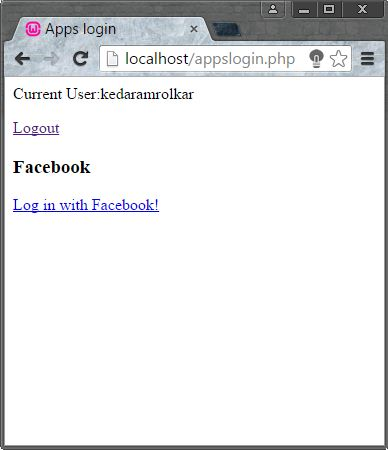
\includegraphics{loginfB}
  \caption{Facebook Login Page}
\end{figure}

\begin{figure}
  \centering
  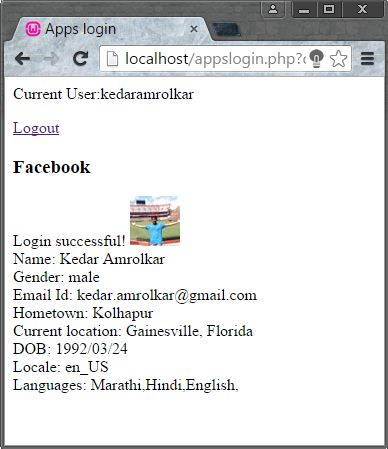
\includegraphics{fBdata}
  \caption{User Data retreived from Facebook}
\end{figure}

\section{Problem and Solution}
Our main aim is to generate awareness among OSN users about the concept of social footprinting. While a user may be aware of the risk of disclosing information on a single OSN, he would most probably not be aware that profile information across multiple OSNs can be aggregated to generate a more comprehensive list of user information. As mentioned in \cite{emergingthreat}, while a user may disclose 4 unique fields in a single OSN, this number doubles when he is a user of five OSNs. This information can then be exploited by miscreants and criminals to cause harm to the user. This may range from offences such as harassment or stalking to crimes such as identity theft. \\

To solve this problem, we first need to collect aggregated data from a user spanning across his multiple social network accounts to build his social footprint. We will achieve this using the APIs exposed by these OSNs. We have so far integrated our application with the Facebook API to pull a users profile data. We aim to use this approach for more popular OSNs which have a large user base. These include Google+ which is similar to Facebook. We then have Twitter which might provide a list of persons that the user might be folllowing signifyng an ideological similarity. Instagram is a photo sharing website that may have its own set of interesting data. LinkedIn is extremely important as a professional network and exposes a different kind of data. SoundCloud would list music preferences and so on.\\

Figures 1 and 2 show a rudimentary functioning of the Facebook API integration.Following this integration, the retrieved data is stored in our database where it will await more data from other OSNs. Repeated data can be ignored. The new data can be aggregated with what has been found so far.\\

Once we have built a footprint, we need to measure its weight. In order to do this, we must have weights associated with all the attributes of a users profile data. We propose to assign these weights based on empirical estimates derived from criminal records. We will list out which attributes contribute the most towards a cybercrime caused by data leakage via public profiles. These attributes will have higher weights. This is a significant challenge as this data is not only crucial to build the mathematical model, it is also very difficult to collect. We have so far scanned over various online resources and collected some numbers. However, it would be important to find and utilize a consolidated data source of crime records and causes. We will continue looking for such data and at the same time, build our weight function using external online sources.\\

Table 1 illustrates the weight table we have built so far. We will keep extending on it as and when we encounter new attributes or identify weights for known attributes from crime records.\\

Based on the weights assigned to attributes, we will compute the aggregated weight of the social footprint. This weight can be calculated trivially as the sum of the weights of all the attributes that have aggregated into the footprint. Then comes the challenge of identifying the risk associated with that footprint. We need to identify a threshold value beyond which the weight of a social footprint would classify as at-risk. We intend to assign a trivial random value for this due to the time constraints. However, this value should be calculated by observing crime patterns as well.\\

Our next task will involve identifying ways to reduce the weight of a social footprint. In this step, the user will be suggested various attributes that could be left out or hidden from his public profile. These suggestions will be made based on the weight of these attributes, and the objective will be to minimize the footprint weight by leaving out these heavy attributes that may cause harm to a user by disclosing it as a public profile attribute.

% The \label must come after \caption as always.

\begin{table}[!t]
\renewcommand{\arraystretch}{3.0}
\caption{Attribute Weights based on Crime Records}
\label{attribute_table}
\centering
\begin{tabular}{|c||c|}
\hline
\large{First Name} & \large{1}\\
\hline
\large{Second Name} & \large{1}\\
\hline
\large{Middle Name} & \large{1}\\
\hline
\large{Age} & \large{1}\\
\hline
\large{Sex} & \large{1}\\
\hline

\end{tabular}
\end{table}

\section{Roadmap for remaining work}
\subsection{Collecting footprint data from more OSNs}
The increase in OSNs coupled with the boom in API integrations gives us a rich source of information. We are hoping to integrate the tool with as many Social Networks via their APIs as possible. These will also span various domains - while Facebook may have most of the information that contributes to a footprint, there are many other interesting OSNs today that may contain interesting bits of information that could increase the weight of a footprint. LinkedIn will have professional information about a person which may help draw inferences about his travel routes, work hours and most importantly, income. We also have intersting OSNs such as Pinterest which is an easy listing of personal interests. Photo sharing sites such as Instagram and music preference sites such as SoundCloud can further help somebody maliciously gain personal information. From our perspective, it is helpful that these OSNs usually expose APIs for developers to integrate with them. This provides us an easy way to pull data for our experiments.
\subsection{API Integration}
The technology stack that we use for the web application is Apache as the server, PHP for the server side scripting and MySQL as the database. PHP being the choice to integrate with as many APIs as possible. No prior experience with PHP comes as a significant challenge to us and is a very important hurdle to overcome as this is the selected source way of collecting footprints for us. This slows down our process of collecting data from multiple sites and buiding the social footprints. However, we have integrated with Facebook which should be very helpful in building forward and integrating with more OSNs. Once we integrate with multiple OSNs, a user will access the web application and then provide his authentication for all the OSNs that he uses. This is needed to call the API to fetch that users data. On retrieving the data from a single OSN, we can store it in a database.The user can then continue to authenticate himself for one OSN after the other, and we can access his data and aggregate it in the database. Once, all the data is collected we can retrieve the entire footprint to calculate the weight.
\subsection{Assigning attribute weights}
We then have to solve the problem of associating weights with these attributes. Prior works assign these weights based on intuition with no real well defined meaning to these weights. We propose that these weights should be based on how the attribute leakage has already harmed users historically. Consider a popular attack in the past where a user might have disclosed his mothers maiden name as a public profile field. This is a popular security question on most websites. This makes the attribute heavy, that is, it would contribute more towards making a social footprint vulnerable. At the same time, disclosing your first name is not as risky as it cannot be used much with a malicious intent. However, aggregated attributes may have more weightage. For example, the first name, last name and date of birth together can create a vulnerable footprint. While these attributes individually are safe to disclose, when they are disclosed together they can be used effectively in identity theft. This in some ways explains how aggregated data is more dangerous than data on a single social network. For an attacker, an aggregated footprint provides much more information and means to cause harm than the data on an individual social networking site. Another aspect in attributes is identifying a person more preecisely. Some attributes such as age and sex may seem generic but these are useful in guaranteeing that the person is the same across multiple OSNs. This helps in creating a social footprint again, which makes these attributes risky to disclose in a group.
\subsection{Calculate and compare with threshold}
After having a list of assigned values for different attributes, we then calculate the weight for that users footprint. We must check what attributes are present in the users footprint. According to that we will fetch those attriute weights and do a simple sum on those weights. This will amount to the total weight of that footprint.
Mathematically, this can be represented as,
\begin{equation}
w(footprint) = \sum_{i=1}^{n}attribute_i
\end{equation}
\subsection{Check for vulnerability}
After we calculate the weight of the footprint, we compare it to a threshold value to check if it is vulnerable. We plan to do this simply by considering the average footprint weights of five users who can be considered to have safe footprints. That is, these users will be having very minimal public profile attributes which guarantee bare minimum visibility on these websites. This average footprint weight will be considered as the threshold for our remaining checks. While this is crude as compared to some previous works as in \cite{pidx}, it will temporariliy accomplish the requirements and we can extend on this approach when time permits.
\subsection{Suggestion reduction in weights}
Once we have the threshold value and the result of the comparison with that value, we can determine the vulnerability of the footprint. In simple words if the footprint weight crosses the threshold value, it is vulnerable and we must bring the footprint weight down below the threshold. In order to achieve this, some attributes need to be removed from the users footprint or effectively from their OSN profile. This must be done keeping in mind that visibility must not be reduced drastically. We need to minimize the weight of the footprint and at the same time keep the visibility constant. While this is a classic linear programming problem, we will simply provide suggestions to users in decreasing order of weight of attributes. Considering that the weights will be assigned keeping in mind visibility, we can assume that heavy attributes will also be ones that will be affecting visibility less. The user can then decide if he wants to modify his profile or not. We will only provide suggestions.

\section{Conclusion}
We attempt to highlight the dangers of disclosing a range of personal data via public profile attributes on online social networks. We will build a social footprint of an individual by accessing his public and other profile data across various OSNs and aggregating them. We will then calculate this footprint weight by assigning weights to these attributes. The weights will be based on the risk measure of the attributes by observing past crime patterns related to OSNs over the past few years. By comparing this footprint to a threshold value, we will then determine the level of risk a person is subject to with his current OSN's public and other profile data. Following this we can provide suggestions to reduce the public and other data and trim the weight of the footprint.

% trigger a \newpage just before the given reference
% number - used to balance the columns on the last page
% adjust value as needed - may need to be readjusted if
% the document is modified later
%\IEEEtriggeratref{8}
% The "triggered" command can be changed if desired:
%\IEEEtriggercmd{\enlargethispage{-5in}}

\begin{thebibliography}{1}
\bibitem{emergingthreat} 		%introduction of concept of different fields from different sites
Danesh Irani, Steve Webb, Kang Li, Calton Pu: 
\textit{Large Online Social Footprints -An Emerging Threat}. 
 
\bibitem{leakage}		% a good math representation of bits leakage from different places
Danesh Irani, Steve Webb, Calton Pu, Kang Li: 
\textit{Modeling Unintended Personal-Information Leakage from Multiple Online Social Networks}
 
\bibitem{privacypaper} %study leakage from different sites from the view point of third party apps accessing data
Balachander Krishnamurthy, Craig E. Wills: 
\textit{Characterizing Privacy in Online Social Networks}

\bibitem{inforevelation}	%early paper for CMU students amount of info revelation
Ralph Gross, Alessandro Acquisti: 
\textit{Information Revelation and Privacy in Online Social Networks}

\bibitem{undermining}	%possible threats and solutions for privacy leak 
Monica Chew, Dirk Balfanz, Ben Laurie: 
\textit{(Under)mining Privacy in Social Networks}

\bibitem{pidx}	% a good math representation pidx should try to incorporate
Yong Wang, Raj Kumar Nepali, Jason Nikolai: 
\textit{Social Network Privacy Measurement and Simulation}

\bibitem{paas} %framework for data collection and representation
E. Michael Maximilien, Tyrone Grandison, Tony Sun, Dwayne Richardson, Sherry Guo, Kun Liu: 
\textit{Privacy-as-a-Service: Models, Algorithms, and Results on the Facebook Platform}

\bibitem{privometer}	%facebook tool for privacy risk by accessing all data
Nilothpal Talukder, Mourad Ouzzani, Ahmed K. Elmagarmid, Hazem Elmeleegy, and Mohamed Yakout: 
\textit{Privometer: Privacy Protection in Social Networks}

\bibitem{socialgraph}	% understand risk based on items disclosed
Cuneyt Gurcan Akcora, Barbara Carminati, Elena Ferrari: 
\textit{Privacy in Social Networks: How Risky is Your Social Graph?}

\bibitem{framework}	%privacy score calculated on sensitivity of data and risk associated with it
Kun Liu, Evimaria Terzi: 
\textit{A Framework for Computing the Privacy Scores of Users in Online Social Networks}

\bibitem{privaware}	%calculate privacy risk and gather user sentiment about it Facebook only
Justin Becker, Hao Chen: 
\textit{Measuring Privacy Risk in Online Social Networks}

\bibitem{census}	%stats on profile attributes
L.Sweeney: 
\textit{Uniqueness of Simple Demographics in The US Population}

\bibitem{statswebsite} 
Statistics Portal at statista.com
\\\texttt{\url{http://www.statista.com/topics/1164/social-networks/}}

\bibitem{newsarticle} 
Socialnomics
\\\texttt{\url{http://www.socialnomics.net/2014/03/04/the-shocking-truth-about-social-networking-crime/}}


%\begin{figure}[!t]
%\centering
%\includegraphics[width=2.5in]{myfigure}
% where an .eps filename suffix will be assumed under latex, 
% and a .pdf suffix will be assumed for pdflatex; or what has been declared
% via \DeclareGraphicsExtensions.
%\caption{Simulation results for the network.}
%\label{fig_sim}
%\end{figure}


% An example of a double column floating figure using two subfigures.
% (The subfig.sty package must be loaded for this to work.)
% The subfigure \label commands are set within each subfloat command,
% and the \label for the overall figure must come after \caption.
% \hfil is used as a separator to get equal spacing.
% Watch out that the combined width of all the subfigures on a 
% line do not exceed the text width or a line break will occur.
%
%\begin{figure*}[!t]
%\centering
%\subfloat[Case I]{\includegraphics[width=2.5in]{box}%
%\label{fig_first_case}}
%\hfil
%\subfloat[Case II]{\includegraphics[width=2.5in]{box}%
%\label{fig_second_case}}
%\caption{Simulation results for the network.}
%\label{fig_sim}
%\end{figure*}
%


%\usepackage{stfloats}
% stfloats.sty was written by Sigitas Tolusis. This package gives LaTeX2e
% the ability to do double column floats at the bottom of the page as well
% as the top. (e.g., "\begin{figure*}[!b]" is not normally possible in
% LaTeX2e). It also provides a command:
%\fnbelowfloat
% to enable the placement of footnotes below bottom floats (the standard
% LaTeX2e kernel puts them above bottom floats). This is an invasive package
% which rewrites many portions of the LaTeX2e float routines. It may not work
% with other packages that modify the LaTeX2e float routines. The latest
% version and documentation can be obtained at:
% http://www.ctan.org/pkg/stfloats
% Do not use the stfloats baselinefloat ability as the IEEE does not allow
% \baselineskip to stretch. Authors submitting work to the IEEE should note
% that the IEEE rarely uses double column equations and that authors should try
% to avoid such use. Do not be tempted to use the cuted.sty or midfloat.sty
% packages (also by Sigitas Tolusis) as the IEEE does not format its papers in
% such ways.
% Do not attempt to use stfloats with fixltx2e as they are incompatible.
% Instead, use Morten Hogholm'a dblfloatfix which combines the features
% of both fixltx2e and stfloats:
%
% \usepackage{dblfloatfix}

% *** MISC UTILITY PACKAGES ***
%
%\usepackage{ifpdf}
% Heiko Oberdiek's ifpdf.sty is very useful if you need conditional
% compilation based on whether the output is pdf or dvi.
% usage:
% \ifpdf
%   % pdf code
% \else
%   % dvi code
% \fi
% The latest version of ifpdf.sty can be obtained from:
% http://www.ctan.org/pkg/ifpdf
% Also, note that IEEEtran.cls V1.7 and later provides a builtin
% \ifCLASSINFOpdf conditional that works the same way.
% When switching from latex to pdflatex and vice-versa, the compiler may
% have to be run twice to clear warning/error messages.


% *** CITATION PACKAGES ***
%
%\usepackage{cite}
% cite.sty was written by Donald Arseneau
% V1.6 and later of IEEEtran pre-defines the format of the cite.sty package
% \cite{} output to follow that of the IEEE. Loading the cite package will
% result in citation numbers being automatically sorted and properly
% "compressed/ranged". e.g., [1], [9], [2], [7], [5], [6] without using
% cite.sty will become [1], [2], [5]--[7], [9] using cite.sty. cite.sty's
% \cite will automatically add leading space, if needed. Use cite.sty's
% noadjust option (cite.sty V3.8 and later) if you want to turn this off
% such as if a citation ever needs to be enclosed in parenthesis.
% cite.sty is already installed on most LaTeX systems. Be sure and use
% version 5.0 (2009-03-20) and later if using hyperref.sty.
% The latest version can be obtained at:
% http://www.ctan.org/pkg/cite
% The documentation is contained in the cite.sty file itself.

% *** MATH PACKAGES ***
%
%\usepackage{amsmath}
% A popular package from the American Mathematical Society that provides
% many useful and powerful commands for dealing with mathematics.
%
% Note that the amsmath package sets \interdisplaylinepenalty to 10000
% thus preventing page breaks from occurring within multiline equations. Use:
%\interdisplaylinepenalty=2500
% after loading amsmath to restore such page breaks as IEEEtran.cls normally
% does. amsmath.sty is already installed on most LaTeX systems. The latest
% version and documentation can be obtained at:
% http://www.ctan.org/pkg/amsmath

% *** SPECIALIZED LIST PACKAGES ***
%
%\usepackage{algorithmic}
% algorithmic.sty was written by Peter Williams and Rogerio Brito.
% This package provides an algorithmic environment fo describing algorithms.
% You can use the algorithmic environment in-text or within a figure
% environment to provide for a floating algorithm. Do NOT use the algorithm
% floating environment provided by algorithm.sty (by the same authors) or
% algorithm2e.sty (by Christophe Fiorio) as the IEEE does not use dedicated
% algorithm float types and packages that provide these will not provide
% correct IEEE style captions. The latest version and documentation of
% algorithmic.sty can be obtained at:
% http://www.ctan.org/pkg/algorithms
% Also of interest may be the (relatively newer and more customizable)
% algorithmicx.sty package by Szasz Janos:
% http://www.ctan.org/pkg/algorithmicx


% *** ALIGNMENT PACKAGES ***
%
%\usepackage{array}
% Frank Mittelbach's and David Carlisle's array.sty patches and improves
% the standard LaTeX2e array and tabular environments to provide better
% appearance and additional user controls. As the default LaTeX2e table
% generation code is lacking to the point of almost being broken with
% respect to the quality of the end results, all users are strongly
% advised to use an enhanced (at the very least that provided by array.sty)
% set of table tools. array.sty is already installed on most systems. The
% latest version and documentation can be obtained at:
% http://www.ctan.org/pkg/array

% IEEEtran contains the IEEEeqnarray family of commands that can be used to
% generate multiline equations as well as matrices, tables, etc., of high
% quality.

% *** SUBFIGURE PACKAGES ***
%\ifCLASSOPTIONcompsoc
%  \usepackage[caption=false,font=normalsize,labelfont=sf,textfont=sf]{subfig}
%\else
%  \usepackage[caption=false,font=footnotesize]{subfig}
%\fi
% subfig.sty, written by Steven Douglas Cochran, is the modern replacement
% for subfigure.sty, the latter of which is no longer maintained and is
% incompatible with some LaTeX packages including fixltx2e. However,
% subfig.sty requires and automatically loads Axel Sommerfeldt's caption.sty
% which will override IEEEtran.cls' handling of captions and this will result
% in non-IEEE style figure/table captions. To prevent this problem, be sure
% and invoke subfig.sty's "caption=false" package option (available since
% subfig.sty version 1.3, 2005/06/28) as this is will preserve IEEEtran.cls
% handling of captions.
% Note that the Computer Society format requires a larger sans serif font
% than the serif footnote size font used in traditional IEEE formatting
% and thus the need to invoke different subfig.sty package options depending
% on whether compsoc mode has been enabled.
%
% The latest version and documentation of subfig.sty can be obtained at:
% http://www.ctan.org/pkg/subfig


% *** FLOAT PACKAGES ***
%
%\usepackage{fixltx2e}
% fixltx2e, the successor to the earlier fix2col.sty, was written by
% Frank Mittelbach and David Carlisle. This package corrects a few problems
% in the LaTeX2e kernel, the most notable of which is that in current
% LaTeX2e releases, the ordering of single and double column floats is not
% guaranteed to be preserved. Thus, an unpatched LaTeX2e can allow a
% single column figure to be placed prior to an earlier double column
% figure.
% Be aware that LaTeX2e kernels dated 2015 and later have fixltx2e.sty's
% corrections already built into the system in which case a warning will
% be issued if an attempt is made to load fixltx2e.sty as it is no longer
% needed.
% The latest version and documentation can be found at:
% http://www.ctan.org/pkg/fixltx2e


\end{thebibliography}

\end{document}


